% Chapter 4: Design and Implementation

\chapter{Diseño e implementación} % Main chapter title

\label{Chapter4} % Reference

%----------------------------------------------------------------------------------------

\section{Arquitectura de seguridad}

Para entender la arquitectura de seguridad de la aplicación, es importante
distinguir entre las siguientes propiedades de la seguridad de la información:
confidencialidad, integridad y autenticación.
%Para desarrollar este punto, la sección se va a dividir en las distintas
%propiedades de la seguridad de la información que posee la aplicación:

\subsection{Confidencialidad}

%Desde un principio se pensó en criptografía de clave simétrica para el cifrado
%de la información. Y, debido a su buena reputación, AES como algoritmo de
%cifrado.
Para el cifrado de la información se utiliza criptografía de clave simétrica, ya
que ofrece una mayor velocidad de cifrado frente a otros modelos. Debido a que
puede funcionar tanto sobre hardware como sobre software, a que es un estándar
del cifrado simétrico y a que no tiene debilidades conocidas, AES es el
algoritmo de cifrado simétrico que se utiliza en esta aplicación.
(Véase~\ref{AES})

De entre todos los tamaños de clave disponibles se ha optado por el de
128 bits, ya que ofrece un nivel de seguridad adecuado para la aplicación.
Además, un nivel superior habría supuesto una mayor carga computacional.

Igualmente, es necesario cifrar la clave simétrica utilizada. Para ello se
utiliza un sistema de cifrado asimétrico para proteger la clave. Debido otra vez
a su estandarización, se utiliza RSA como algoritmo de cifrado asimétrico.
(Véase~\ref{RSA})

Ya que el número de operaciones de cifrado asimétrico es menor que el del
simétrico, se utiliza el tamaño máximo para una clave RSA: 4096 bits.

\subsection{Integridad}

%También era importante que el contenido del mensaje permaneciese intacto. Para
%ello había que incluir algún mecanismo de resumen que nos asegurase la
%integridad del mensaje.
También es importante que el mensaje permanezca íntegro. Para ello se ha
incluido un mecanismo de resumen.

De entre algunos algoritmos de resumen se ha decidido utilizar PSS. Este
algoritmo, entre otras cosas, combina el uso de una \emph{salt} con un resumen
hash, lo cual lo hace más robusto frente a determinados ataques enfocados en la
obtención del mensaje original a partir de su resumen. (Véase~\ref{PSS})

\subsection{Autenticación}

El destinatario tiene que poder autenticar al autor del mensaje. Para lograrlo
se incluye junto al mensaje una HMAC. (Véase~\ref{HMAC})

Se utiliza como algoritmo de firma RSASSA-PSS, ya que combina los algoritmos
utilizados para preservar la confidencialidad y la integridad. Este algoritmo
codifica el mensaje utilizando para ello PSS y luego firma (cifra) el mensaje
usando RSA. (Véase~\ref{RSASSA-PSS})

%Para proporcionarle aún más seguridad a la firma se decidió convertir la MAC en
%una HMAC, lo que implicó cifrar la MAC con la clave pública del destinatario de
%forma que solo él pudiera acceder a su contenido.
Para proporcionar confidencialidad a la firma, esta va cifrada usando la clave
pública del destinatario, de forma que nadie más pueda acceder a su contenido.

%----------------------------------------------------------------------------------------

\section{Arquitectura del software}

%Para explicar la arquitectura software de la aplicación, esta sección va a
%estar dividida en varios prototipos que se han desarrollado:
El objetivo de este software es proporcionar una herramienta que permita a los
usuarios mantener comunicaciones con otros usuarios preservando las tres
propiedades de la seguridad comentadas en el punto anterior. Para ello, se ha
llevado a cabo el desarrollo de varios prototipos:

\begin{itemize}
  \item El primer prototipo recibe un fichero y lo divide en varios fragmentos
  de un tamaño dado. También puede recomponer el fichero original a partir de
  los fragmentos.

  \item El segundo prototipo realiza las mismas tareas que el anterior, y además
  añade confidencialidad a los fragmentos mediante un sistema de cifrado
  simétrico.

  \item El tercer prototipo realiza las mismas tareas que el anterior, y además
  añade el uso de RSA para cifrar claves simétricas y proporcionar integridad y
  autenticación a los fragmentos.

  \item El cuarto prototipo realiza las mismas tareas que el anterior, ahora
  como una aplicación en Android. Se añade una interfaz gráfica y hace uso de
  algunas herramientas que posee Android para el almacenamiento de claves.
\end{itemize}

\subsection{Shatter I}

El primer prototipo de la aplicación está desarrollado enteramente en Java,
usando para ello el entorno de desarrollo Eclipse. Esta primera versión busca
poder dividir un fichero en varios fragmentos de un tamaño dado, y luego poder
recomponerlo. Para ello se han implementado algunas clases para almacenar los
datos de los fragmentos:

\begin{figure}[!htb]
  \centering
  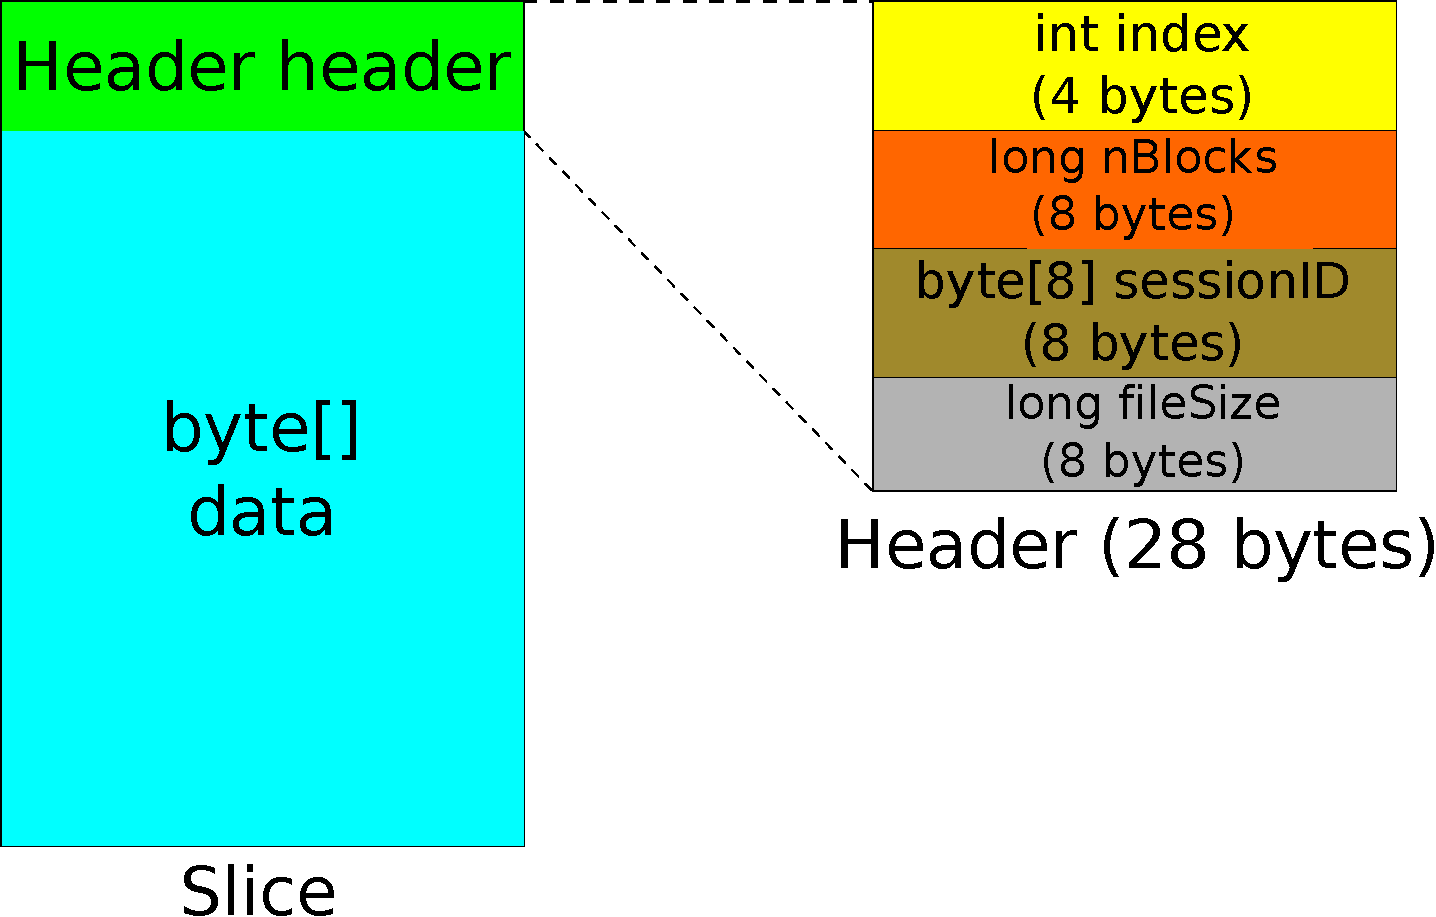
\includegraphics[scale=0.4]{Figures/Slice_Header_1}
  \decoRule
  \caption[Slice - Header (Versión 1)]{Esquema general de las clases Slice y Header (Versión 1)}
  \label{fig:Slice_Header_1}
\end{figure}

\begin{itemize}
  \item \keyword{Slice} -- Un Slice es uno de los fragmentos en los que un
  fichero original se ha dividido. Está formado por una cabecera (Header) y un
  array de bytes en el que se almacena el contenido del segmento del fichero.
  (Figura~\ref{fig:Slice_Header_1})\footnote{Debido al contexto del TFG, se ha
  decidido no usar UML para confeccionar los esquemas expuestos en este
  capítulo.}

  \item \keyword{Header} -- En esta clase se almacenan los metadatos de los
  Slices. Se guardan datos como un contador, el número total de Slices
  para un fichero, un ID para la sesión\footnote{En esta primera iteración de la
  aplicación, el ID para identificar la sesión es un resumen Hash del fichero.}
  y el tamaño original del fichero. (Figura~\ref{fig:Slice_Header_1})
\end{itemize}

También se han desarrollado otras clases con métodos para trocear y recomponer
un fichero:

\begin{figure}[!htb]
  \centering
  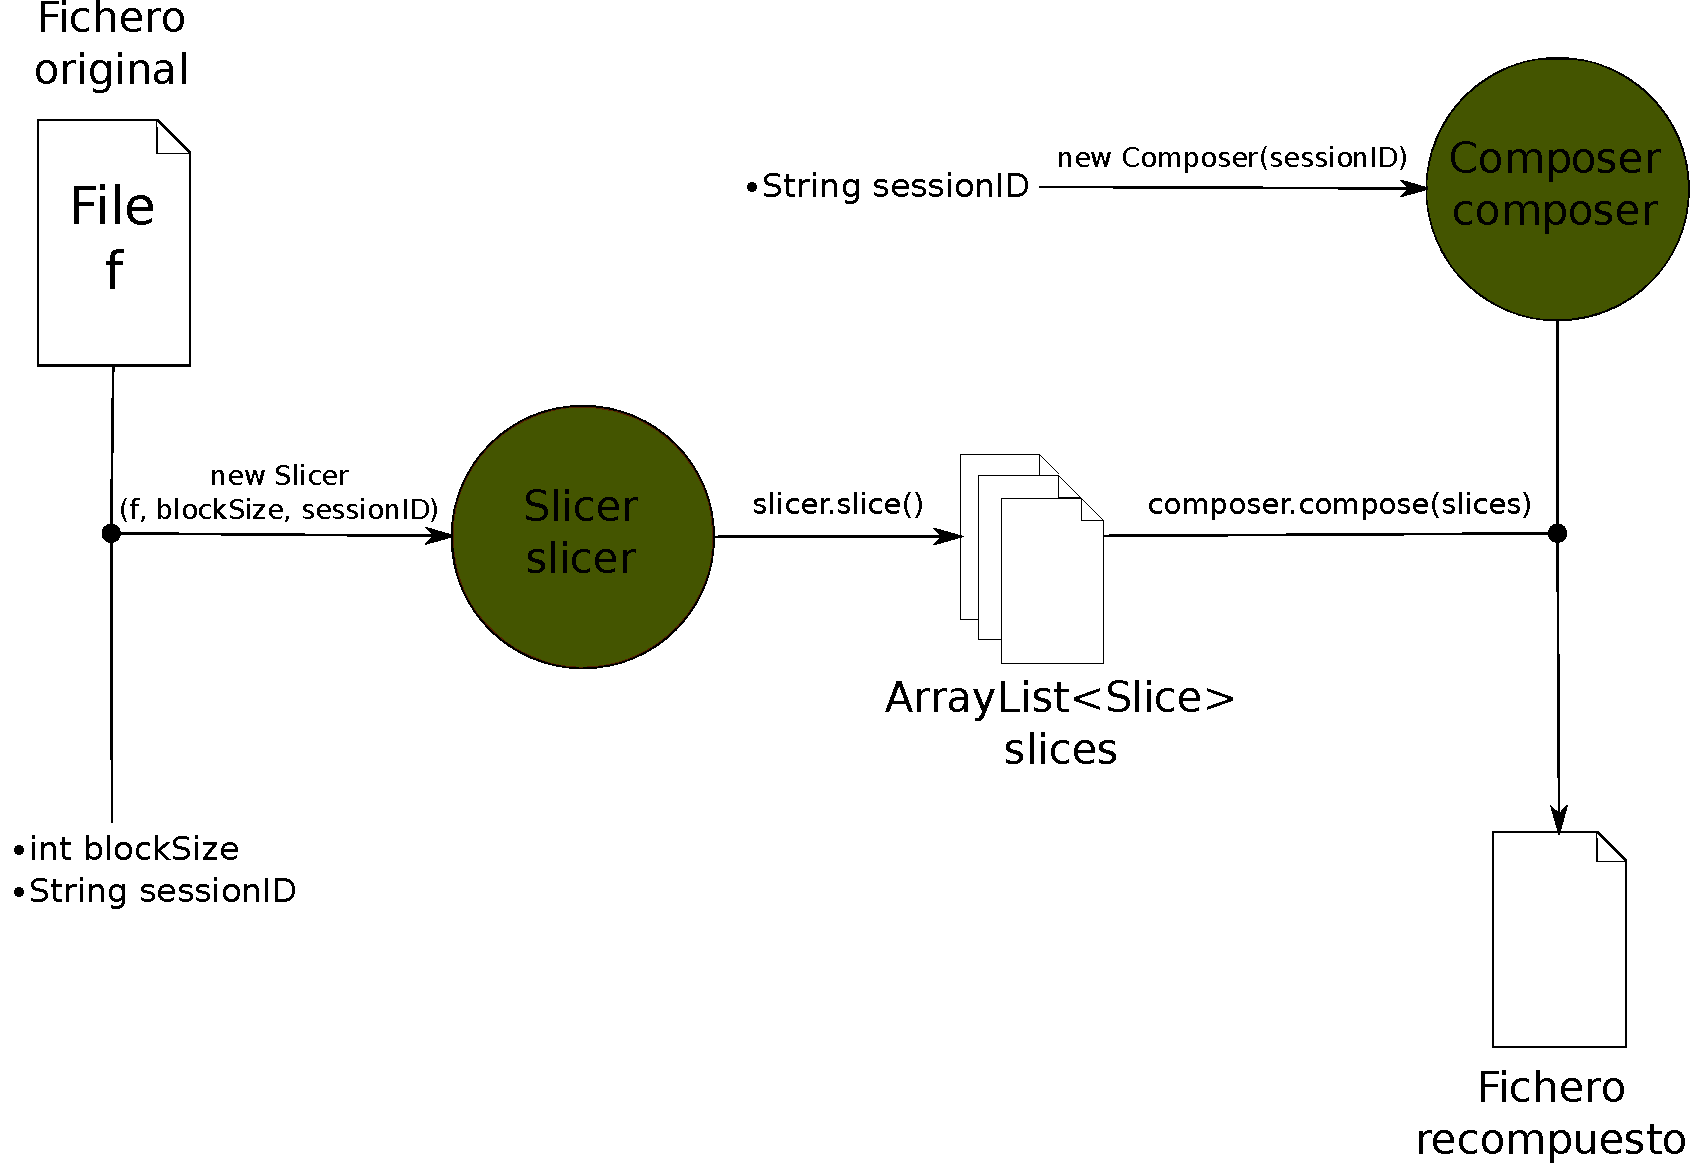
\includegraphics[scale=0.5]{Figures/Assembler}
  \decoRule
  \caption[Slicer - Composer]{Esquema general del Slicer y el Composer}
  \label{fig:Assembler}
\end{figure}

\begin{itemize}
  \item \keyword{Slicer} -- Esta clase posee métodos para crear Slices. Recibe
  un fichero, un tamaño de bloque y un ID para identificar la sesión. Lee del
  fichero bloques del tamaño indicado hasta alcanzar el EOF y genera un Slice
  para cada uno de ellos, con una cabecera distinta.
  (Figura~\ref{fig:Assembler})

  \item \keyword{Composer} -- Esta clase, a través de un método, recibe Slices
  y devuelve un fichero compuesto. Lee uno a uno los Slices que recibe,
  prestando especial atención a sus cabeceras y si detecta que alguno falta
  genera un log de errores. (Figura~\ref{fig:Assembler})
\end{itemize}

%Al tratarse de un prototipo bastante sencillo, no dió muchos problemas, se
%alcanzaron fácilmente los objetivos buscados.

\subsection{Shatter II}

En esta segunda versión, el objetivo del prototipo es proporcionar
confidencialidad a las Slices. Para llevarlo a cabo se han implementado las
siguientes clases:

\begin{figure}[!htb]
  \centering
  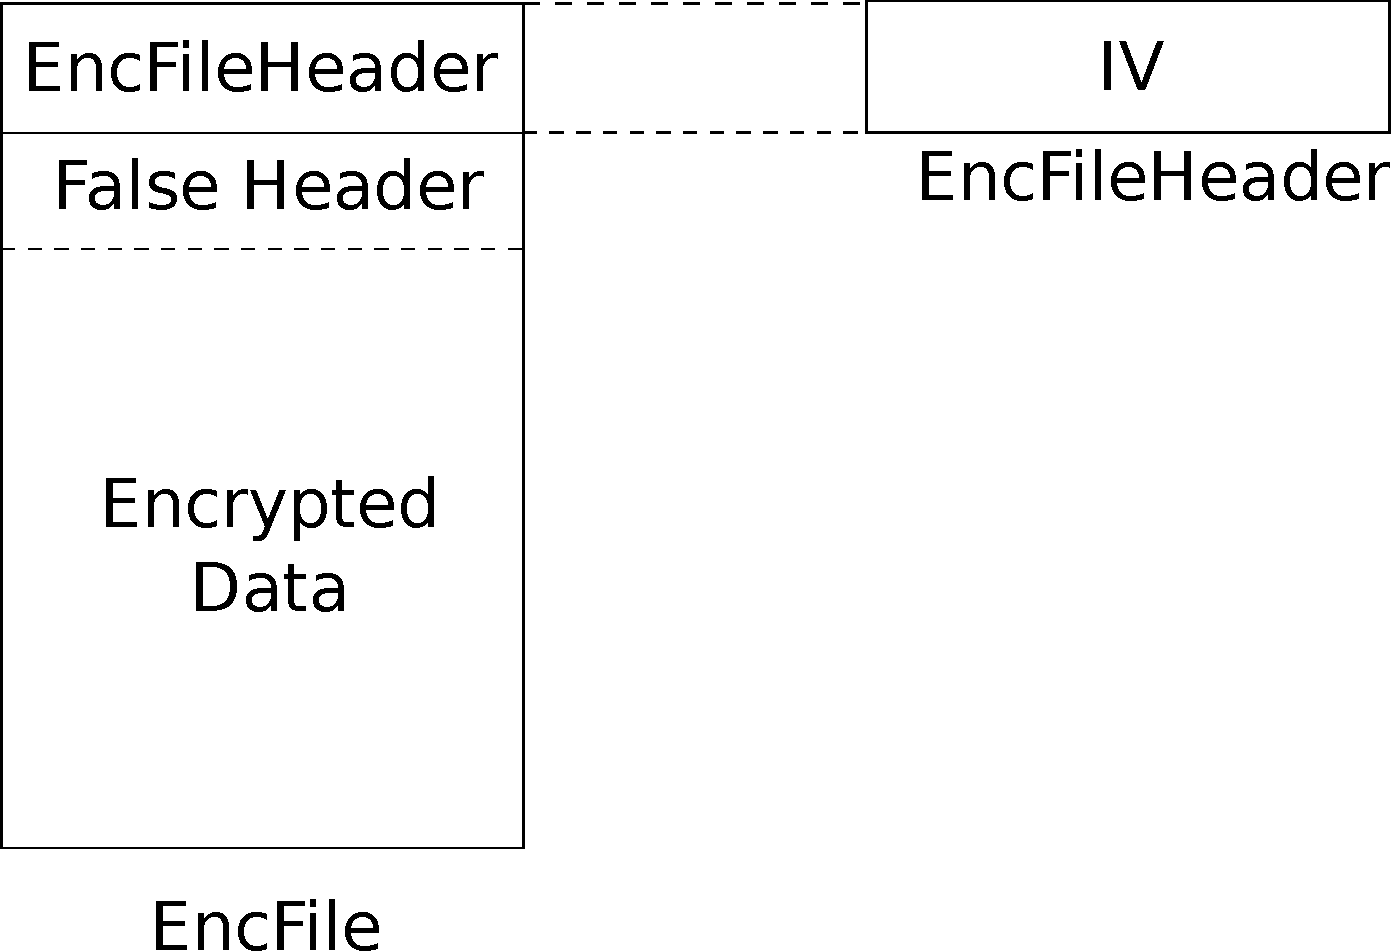
\includegraphics[scale=0.4]{Figures/EncFile_Header_1}
  \decoRule
  \caption[EncFile - EncFileHeader (Versión 1)]{Esquema general de las clases EncFile y EncFileHeader (Versión 1)}
  \label{fig:EncFile_Header_1}
\end{figure}

\begin{itemize}
  \item \keyword{EncFile} -- Viene a ser una Slice cifrada. A parte de los datos
  encriptados de la Slice, también incluye una cabecera (EncFileHeader) con
  algunos datos importantes y una pseudocabecera (FalseHeader) con datos menores.
  (Figura~\ref{fig:EncFile_Header_1})

  \item \keyword{EncFileHeader} -- Esta cabecera se usa para almacenar algunos
  metadatos importantes como, en este caso, el vector de inicialización (IV)
  que se ha usado para cifrar la Slice. (Figura~\ref{fig:EncFile_Header_1})

  \item \keyword{KeyFile} -- Esta clase se utiliza para almacenar la clave
  simétrica que se ha utilizado para crear los EncFiles.
\end{itemize}

Además de estas clases, se han creado otras clases que aportan los métodos
necesarios para cifrar las Slices:

\begin{figure}[!htb]
  \centering
  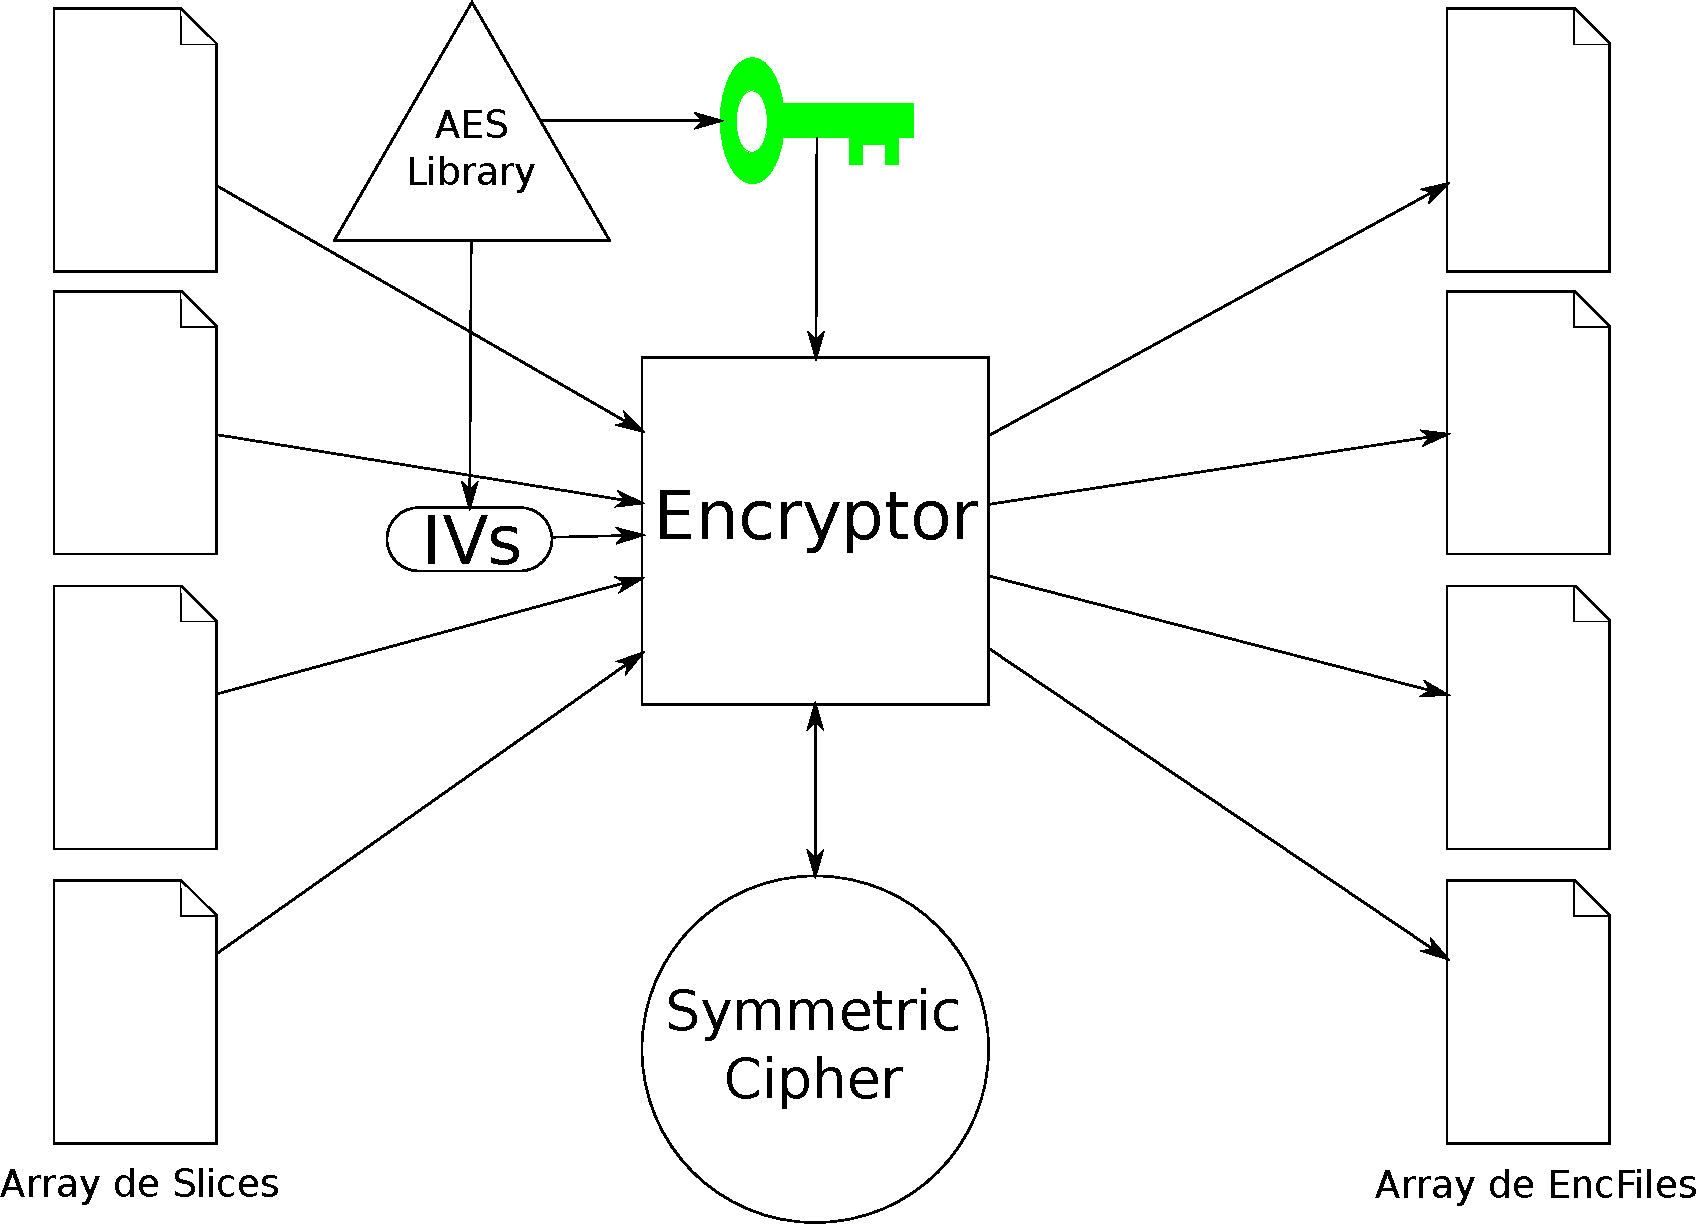
\includegraphics[scale=0.5]{Figures/Encryptor}
  \decoRule
  \caption[Encryptor]{Esquema general del funcionamiento del Encryptor}
  \label{fig:Encryptor}
\end{figure}

\begin{figure}[!htb]
  \centering
  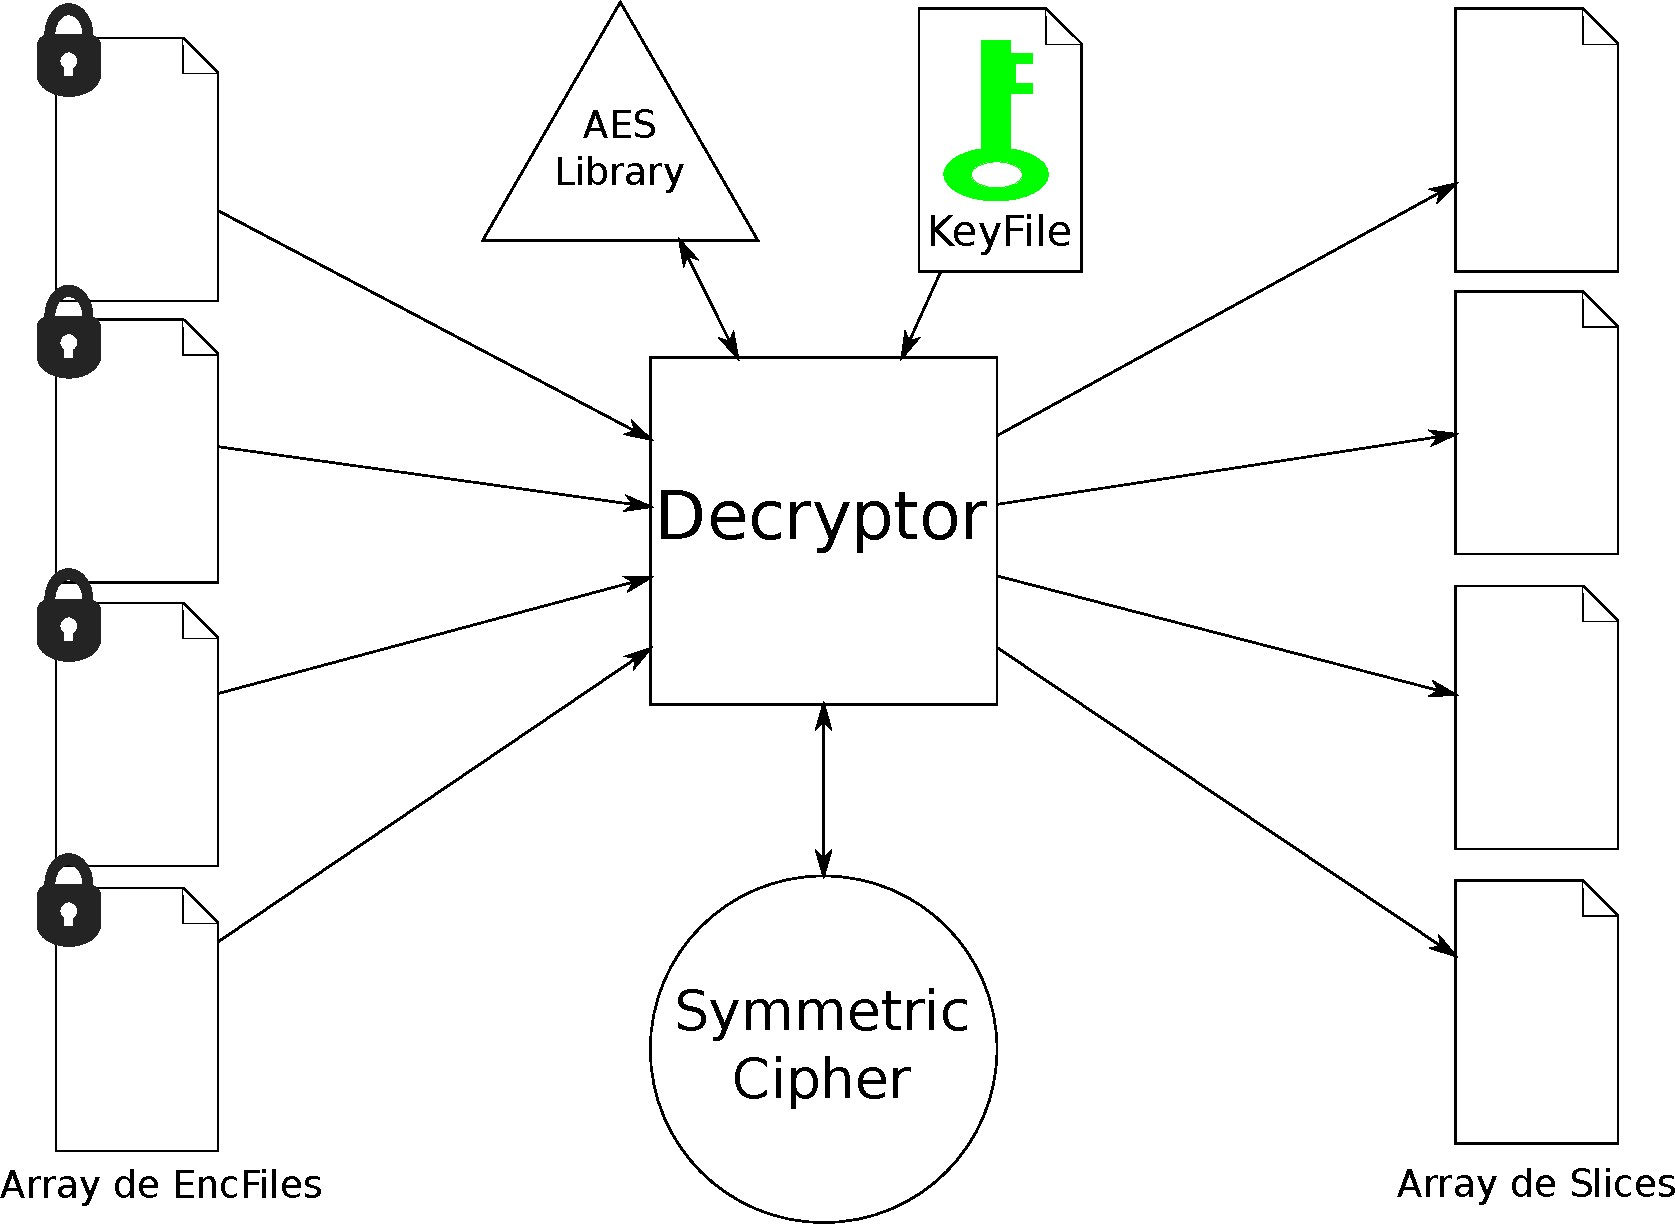
\includegraphics[scale=0.5]{Figures/Decryptor}
  \decoRule
  \caption[Decryptor]{Esquema general del funcionamiento del Decryptor}
  \label{fig:Decryptor}
\end{figure}

\begin{itemize}
  \item \keyword{AESLibrary} -- Básicamente, una clase que se encarga de
  generar de manera aleatoria y segura claves simétricas y vectores de
  inicialización.

  \item \keyword{SymmetricCipher} -- Esta es la clase que se encarga de hacer
  la parte más importante en cuanto a la confidencialidad. Una vez que ha sido
  inicializado con una clave simétrica, genera textos cifrados a partir de
  texto plano y un IV. Igualmente, puede llevar a cabo el proceso inverso.

  \item \keyword{Encryptor} -- Esta clase, en conjunto con las dos anteriores,
  es la encargada de generar los EncFiles. Genera de manera aleatoria y segura
  una clave simétrica para un algoritmo establecido y, con ella, inicializa una
  instancia de un SymmetricCipher. A continuación se le pasa un array de Slices
  del cual genera un array de EncFiles, que es el que devuelve a través de un
  método. (Figura~\ref{fig:Encryptor})

  \item \keyword{Decryptor} -- La contraparte del Encryptor. Realiza el proceso
  inverso y devuelve un array de Slices a partir de uno de EncFiles.
  (Figura~\ref{fig:Decryptor})
\end{itemize}

%A pesar de que la seguridad que proporciona este prototipo no está completa (Ya
%que es propenso a algunos ataques), sienta las bases de lo que será
%la arquitectura de seguridad de la aplicación.

\subsection{Shatter III}

%A pesar de que ya teníamos confidencialidad en las Slices, había que
%proporcionársela también al KeyFile. En este prototipo se crearon las siguientes
%clases para lograrlo:
El objetivo en esta tercera iteración es el de proporcionar integridad y
autenticación a las clases ya están implementadas, al igual que confidencialidad
a la clave simétrica que se utiliza para generarlos. Para lograrlo, se han
implementado algunas clases nuevas:

\begin{itemize}
  \item \keyword{EncKeyFile} -- Esta clase almacena la clave simétrica protegida
  mediante cifrado asimétrico usando la clave pública del destinatario del
  mensaje, con lo que se logra la confidencialidad de la clave entre los
  usuarios. Tiene una cabecera (EncKeyFileHeader) en la que se guardan algunos
  datos importantes.

  \item \keyword{EncKeyFileHeader} -- La cabecera del EncKeyFile. En ella se
  almacena una HMAC cifrada de la clave simétrica.

  \item \keyword{Signature} -- Básicamente una clase para contener una HMAC.

  \item \keyword{SecureSignature} -- Contiene la HMAC comentada antes pero
  cifrada usando una clave asimétrica. De esta forma también le damos
  confidencialidad a la firma.
\end{itemize}

Para poder llevar a cabo el cifrado asimétrico se han desarrollado otras clases:

\begin{figure}[!htb]
  \centering
  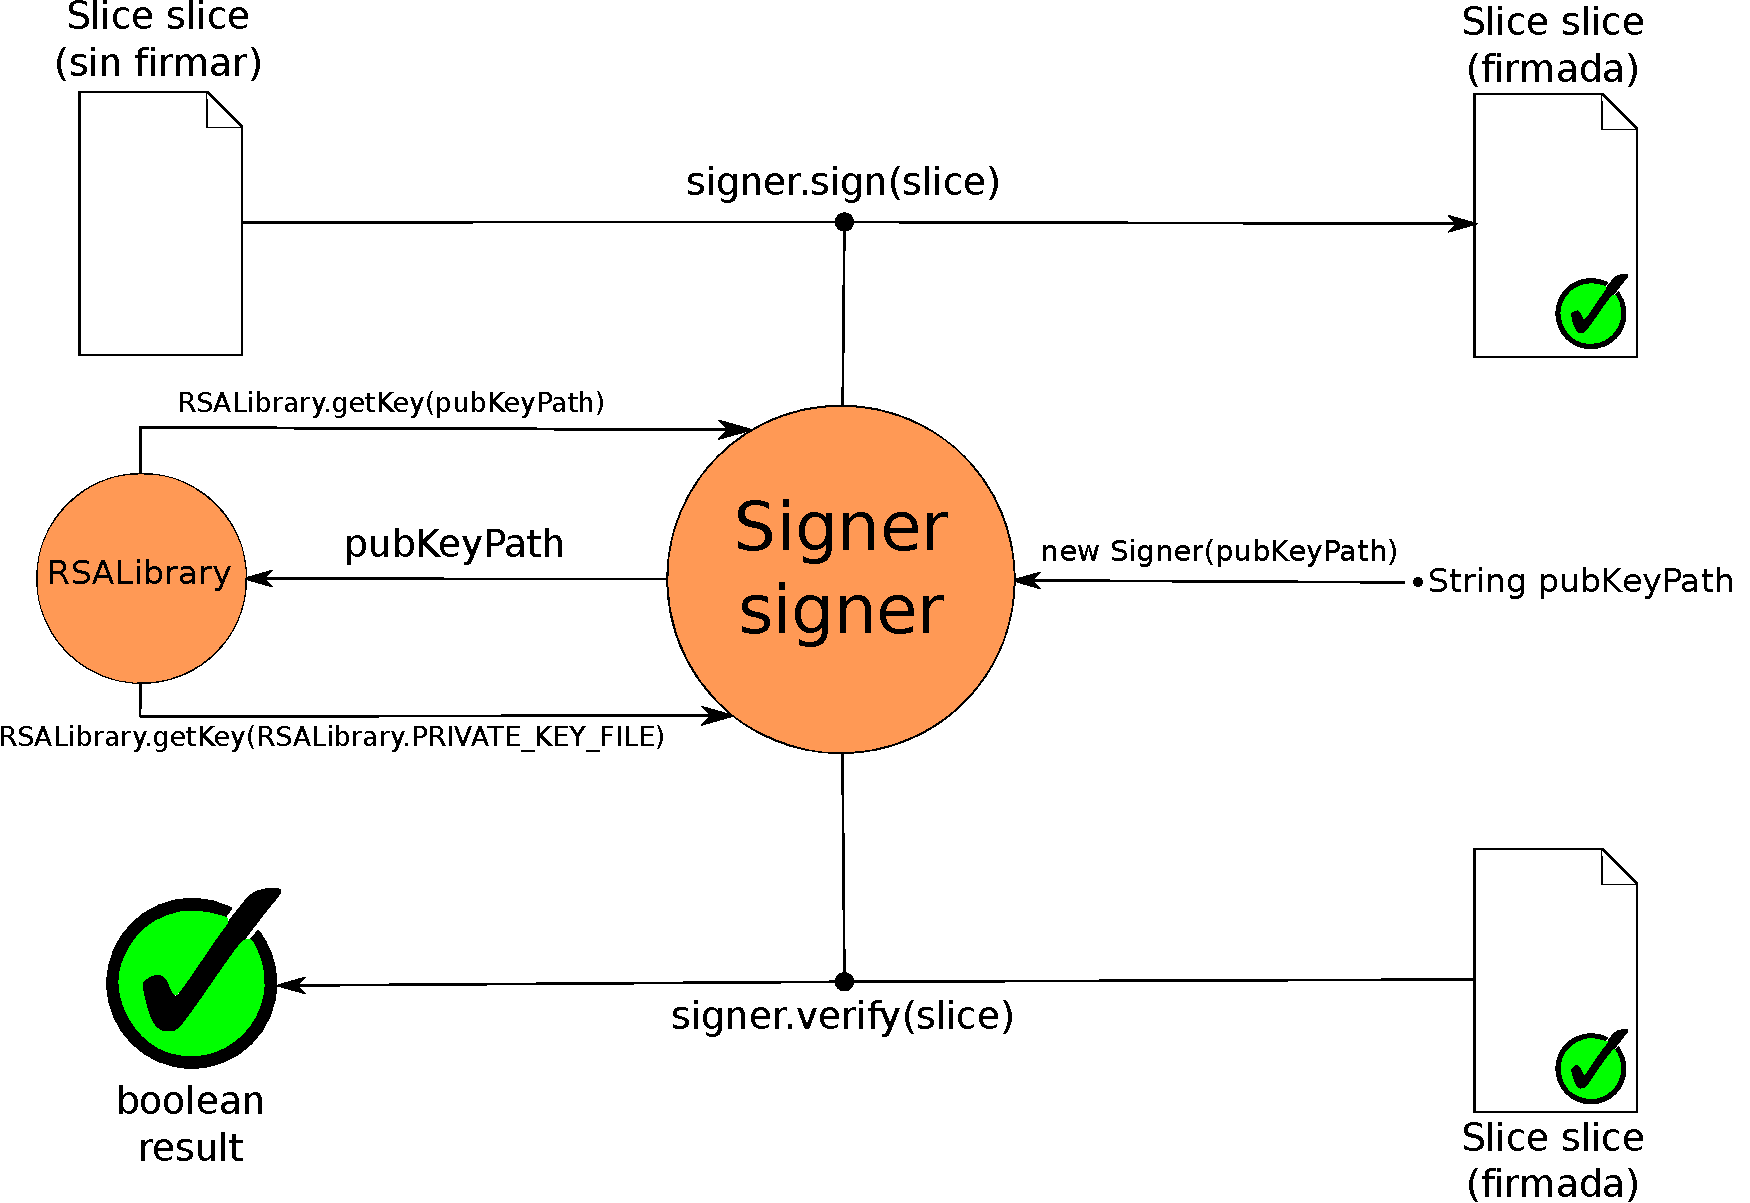
\includegraphics[scale=0.5]{Figures/Signer_1}
  \decoRule
  \caption[Signer (Versión 1)]{Esquema general del funcionamiento del Signer (Versión 1)}
  \label{fig:Signer_1}
\end{figure}

\begin{itemize}
  \item \keyword{RSALibrary} -- Esta clase es la encargada de generar un par de
  claves asimétricas, de escribirlas y leerlas de un fichero y de cifrar
  un texto plano a uno cifrado, y viceversa.

  \item \keyword{Signer} -- La clase que se encarga de recibir Slices, EncFiles,
  KeyFiles y demás y devolverlos firmados. Asimismo, se encarga de comprobar
  las firmas de todos estos ficheros para preservar la autenticidad de la
  información que portan. (Figura~\ref{fig:Signer_1})

  \item \keyword{RSAPSS} -- Esta clase incorpora todos los métodos necesarios
  para generar, a partir de un texto plano, un texto codificado y firmado
  usando el algoritmo RSASSA-PSS. También realiza el proceso inverso y puede
  verificar las firmas.
\end{itemize}

%Con el prototipo anterior nos dimos cuenta de que, aparte de que teníamos que
%generar un modo seguro de transmitir la clave simétrica, también teníamos que
%proporcionar una manera de comprobar la autenticidad de los datos.

%Debido a ello, incluimos una firma en el KeyFile y en las cabeceras de las
%Slices y EncFiles (Figuras~\ref{fig:Slice_Header_2} y~\ref{fig:EncFile_Header_2}).
%Nos dimos cuenta de que algunas firmas iban a ir en claro cuando viajasen de un
%equipo a otro. Por ello se decidió la creación de una firma cifrada (HMAC),
%para evitar posibles "mirones".

En este prototipo se ha añadido una firma a varias de las clases que ya estaban
implementadas:

\begin{figure}[!htb]
  \centering
  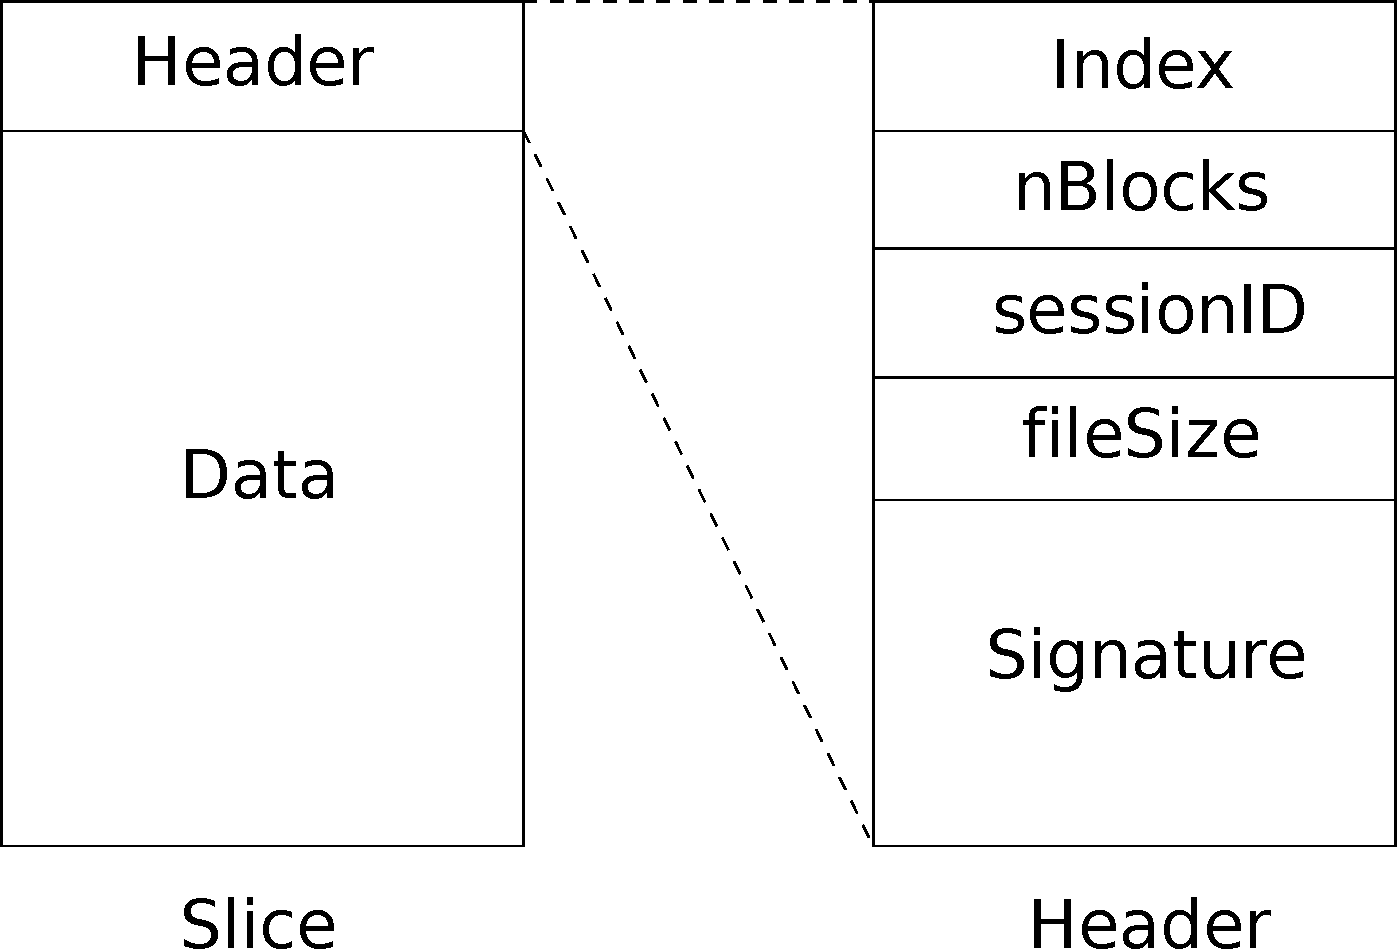
\includegraphics[scale=0.4]{Figures/Slice_Header_2}
  \decoRule
  \caption[Slice - Header (Versión final)]{Esquema general de las clases Slice y Header (Versión final)}
  \label{fig:Slice_Header_2}
\end{figure}

\begin{figure}[!htb]
  \centering
  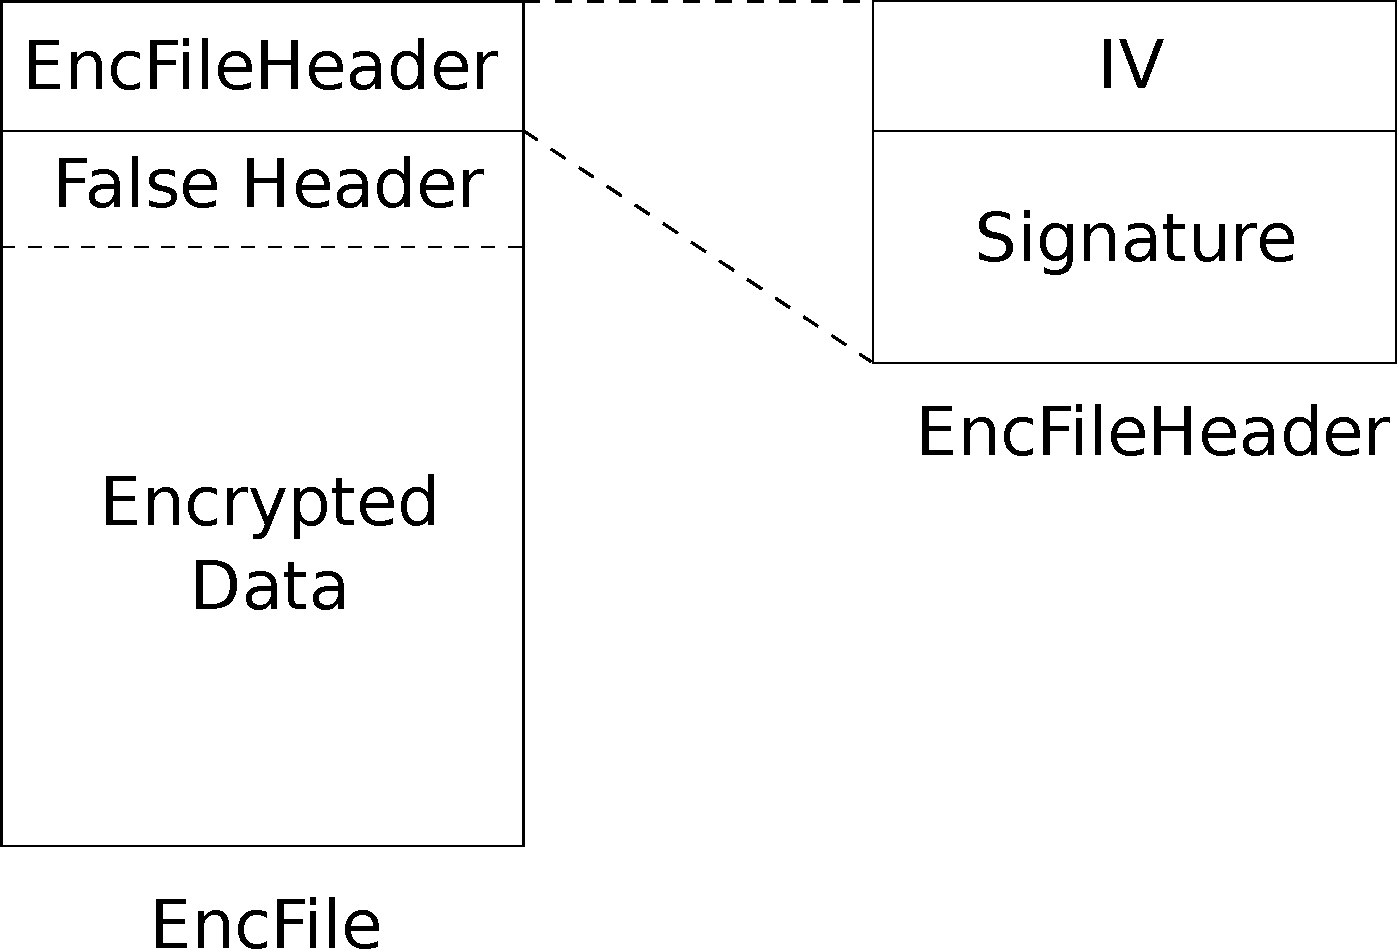
\includegraphics[scale=0.4]{Figures/EncFile_Header_2}
  \decoRule
  \caption[EncFile - EncFileHeader (Versión final)]{Esquema general de las clases EncFile y EncFileHeader (Versión final)}
  \label{fig:EncFile_Header_2}
\end{figure}

\begin{itemize}
  \item A la clase Slice se le ha añadido en la cabecera una firma, que otorga
  integridad y autenticación a los datos que lleva.
  (Figura~\ref{fig:Slice_Header_2})

  \item A la clase EncFile se le ha añadido también una firma, esta vez para
  darle la integridad y la autenticación al IV que se encuentra en su cabecera.
  (Figura~\ref{fig:EncFile_Header_2})

  \item La clase KeyFile tiene una firma de la clave simétrica.
\end{itemize}

Además de las clases mencionadas anteriormente, también se han desarrollado
otras clases funcionales:

\begin{itemize}
  \item \keyword{RandomString} -- Esta clase posee un método que devuelve un
  String aleatorio de 8 caracteres.

  \item \keyword{FileIO} -- Esta clase tiene métodos para escribir y leer los
  distintos ficheros que intervienen en la aplicación.

  \item \keyword{Bytes} -- Tiene implementados varios métodos para hacer
  operaciones con arrays de bytes.
\end{itemize}

\subsection{Shatter IV}

%Esta versión final de la aplicación está marcada por el salto a la plataforma
%Android. Gran parte del código desarrollado en los anteriores prototipos se
%siguió utilizando, sin embargo hubo que cambiar algunas clases:

Este último prototipo está desarrollado como una aplicación en Android. El
objetivo de este prototipo es hacer uso de varias herramientas que posee Android
para que la aplicación funcione correctamente. Para ello se han creado nuevas
clases:

\begin{itemize}
  \item \keyword{KeyStoreHandler} -- Esta clase se usa para realizar todas las
  operaciones necesarias con el Keystore de Android (Véase~\ref{Keystore}). Se
  encarga de almacenar las claves, recuperarlas, usarlas para encriptar,
  firmar, etc.

  \item \keyword{HTTPClient} -- Un cliente HTTP muy sencillo que únicamente
  realiza peticiones GET.

  \item \keyword{ExternalStorage} -- Para interactuar con el External Storage de
  Android se creó una clase que incorpora algunos métodos para conseguir paths,
  descriptores de fichero o crear directorios.
\end{itemize}

%Aparte del desarrollo de estas clases, se trabajó también en un servidor HTTP
%dedicado para almacenar los mensajes enviados por los distintos usuarios de la
%aplicación.

Para que los usuarios puedan enviar sus mensajes, se ha dispuesto un servidor
HTTP bastante sencillo al que los usuarios pueden subir sus mensajes. Gracias a
la clase HTTPClient, el destinatario puede bajarse los fragmentos del mensaje.

%Algunas clases, debido al cambio de plataforma, tuvieron que ser eliminadas.
%El cambio más notorio fue la desaparición de las clases RSALibrary y RSAPSS,
%ambas sustituidas por KeyStoreManager.

\begin{figure}[!htb]
  \centering
  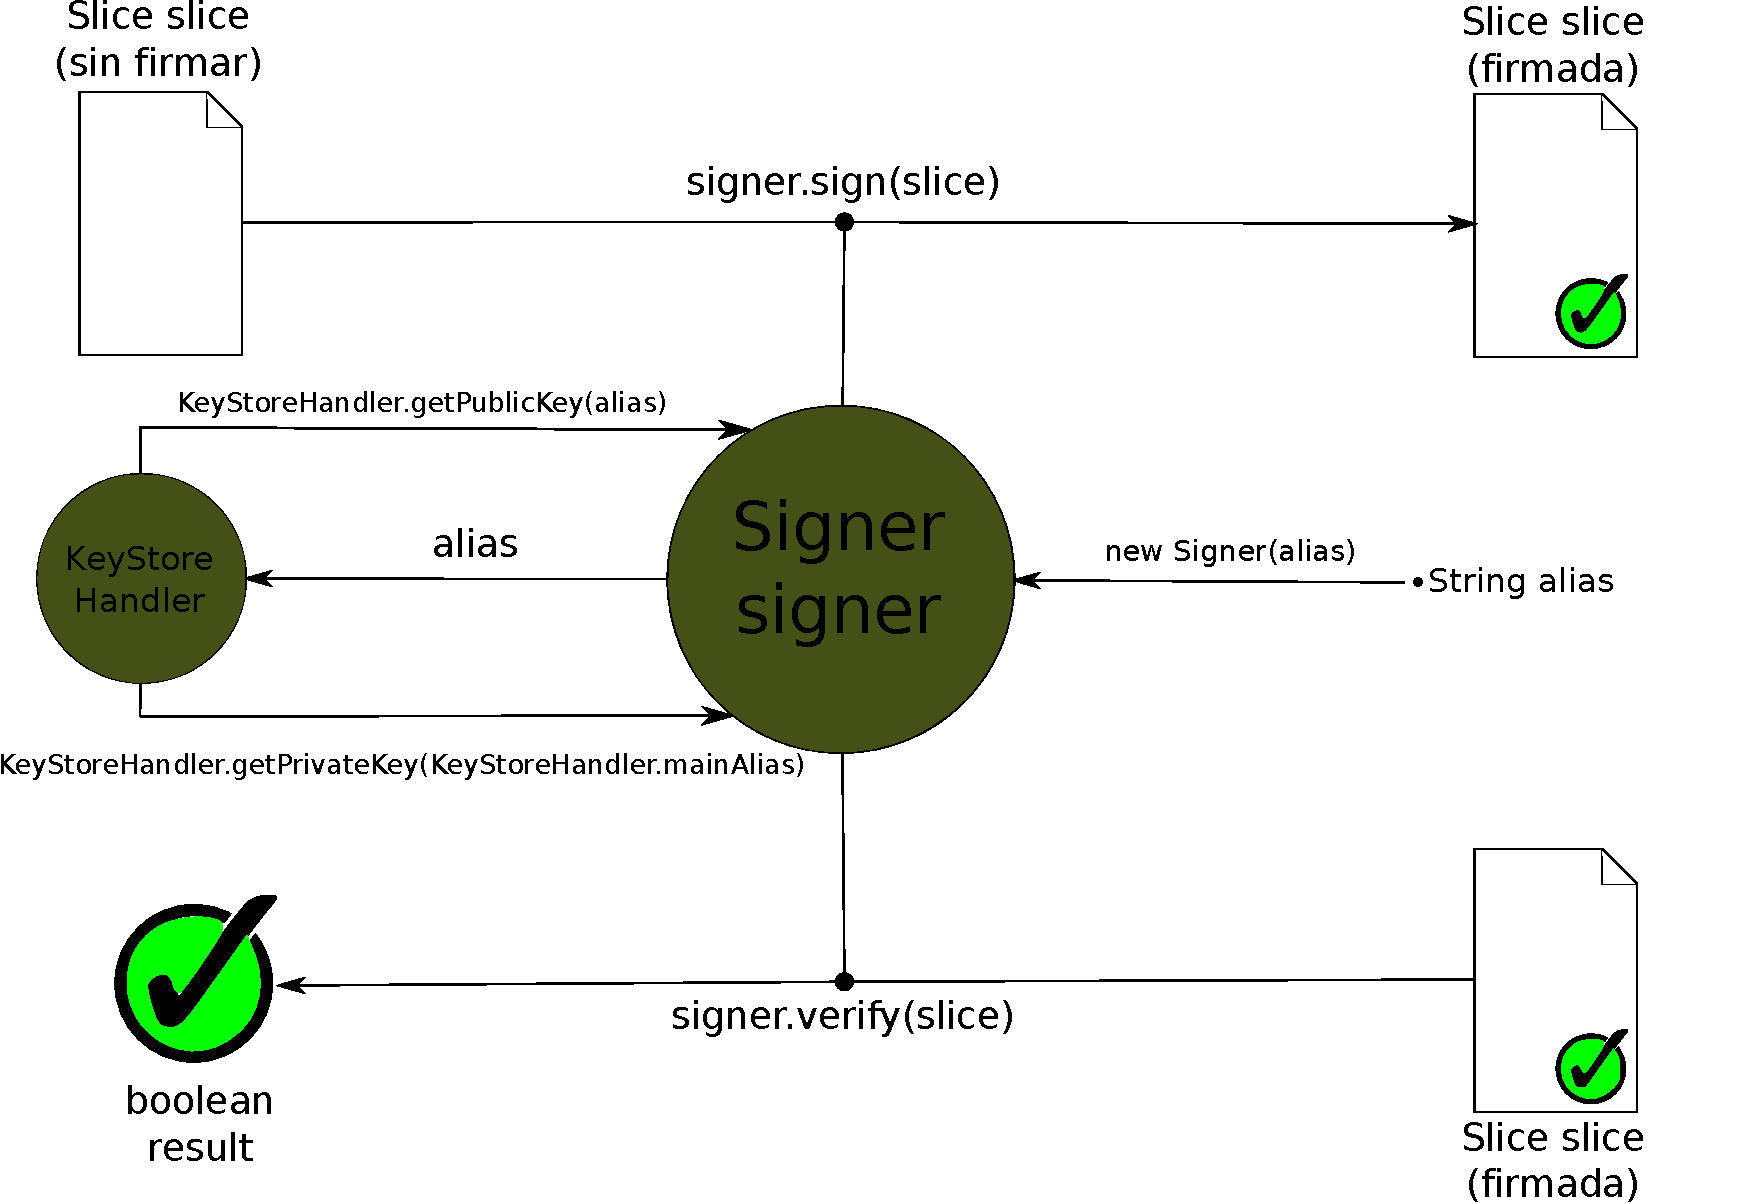
\includegraphics[scale=0.5]{Figures/Signer_2}
  \decoRule
  \caption[Signer (Versión final)]{Esquema general del funcionamiento del Signer (Versión final)}
  \label{fig:Signer_2}
\end{figure}

El uso del Keystore de Android obliga a utilizar las claves que se almacenan en
él usando unos métodos específicos. Debido a ello, algunas clases ya creadas
(Como RSALibrary o RSAPSS) se sustituyen por métodos específicos que se
implementan en la clase KeyStoreHandler. (Figura~\ref{fig:Signer_2})

%Un cambio menor fue la generación de un ID de sesión aleatorio para las
%cabeceras de algunas clases (Anteriormente se usaba un resumen hash del
%fichero).

El ID que aparece en las cabeceras de la clase Slice se sustituye por un String
aleatorio que genera la clase RandomString. Este cambio se debe a que el resumen
hash que se usaba anteriormente queda en desuso al añadir la firma a estas
clases. Además, este ID aleatorio identifica a todas las Slices que pertenecen
a un mismo mensaje.

El esquema general de la aplicación se puede dividir en dos: Una primera parte
se encarga de la división y cifrado del fichero (Figura~\ref{fig:abstractA}). La
otra se encarga de descargar del servidor los fragmentos cifrados y recomponer
el fichero original (Figura~\ref{fig:abstractB}).

\begin{figure}[!htb]
  \centering
  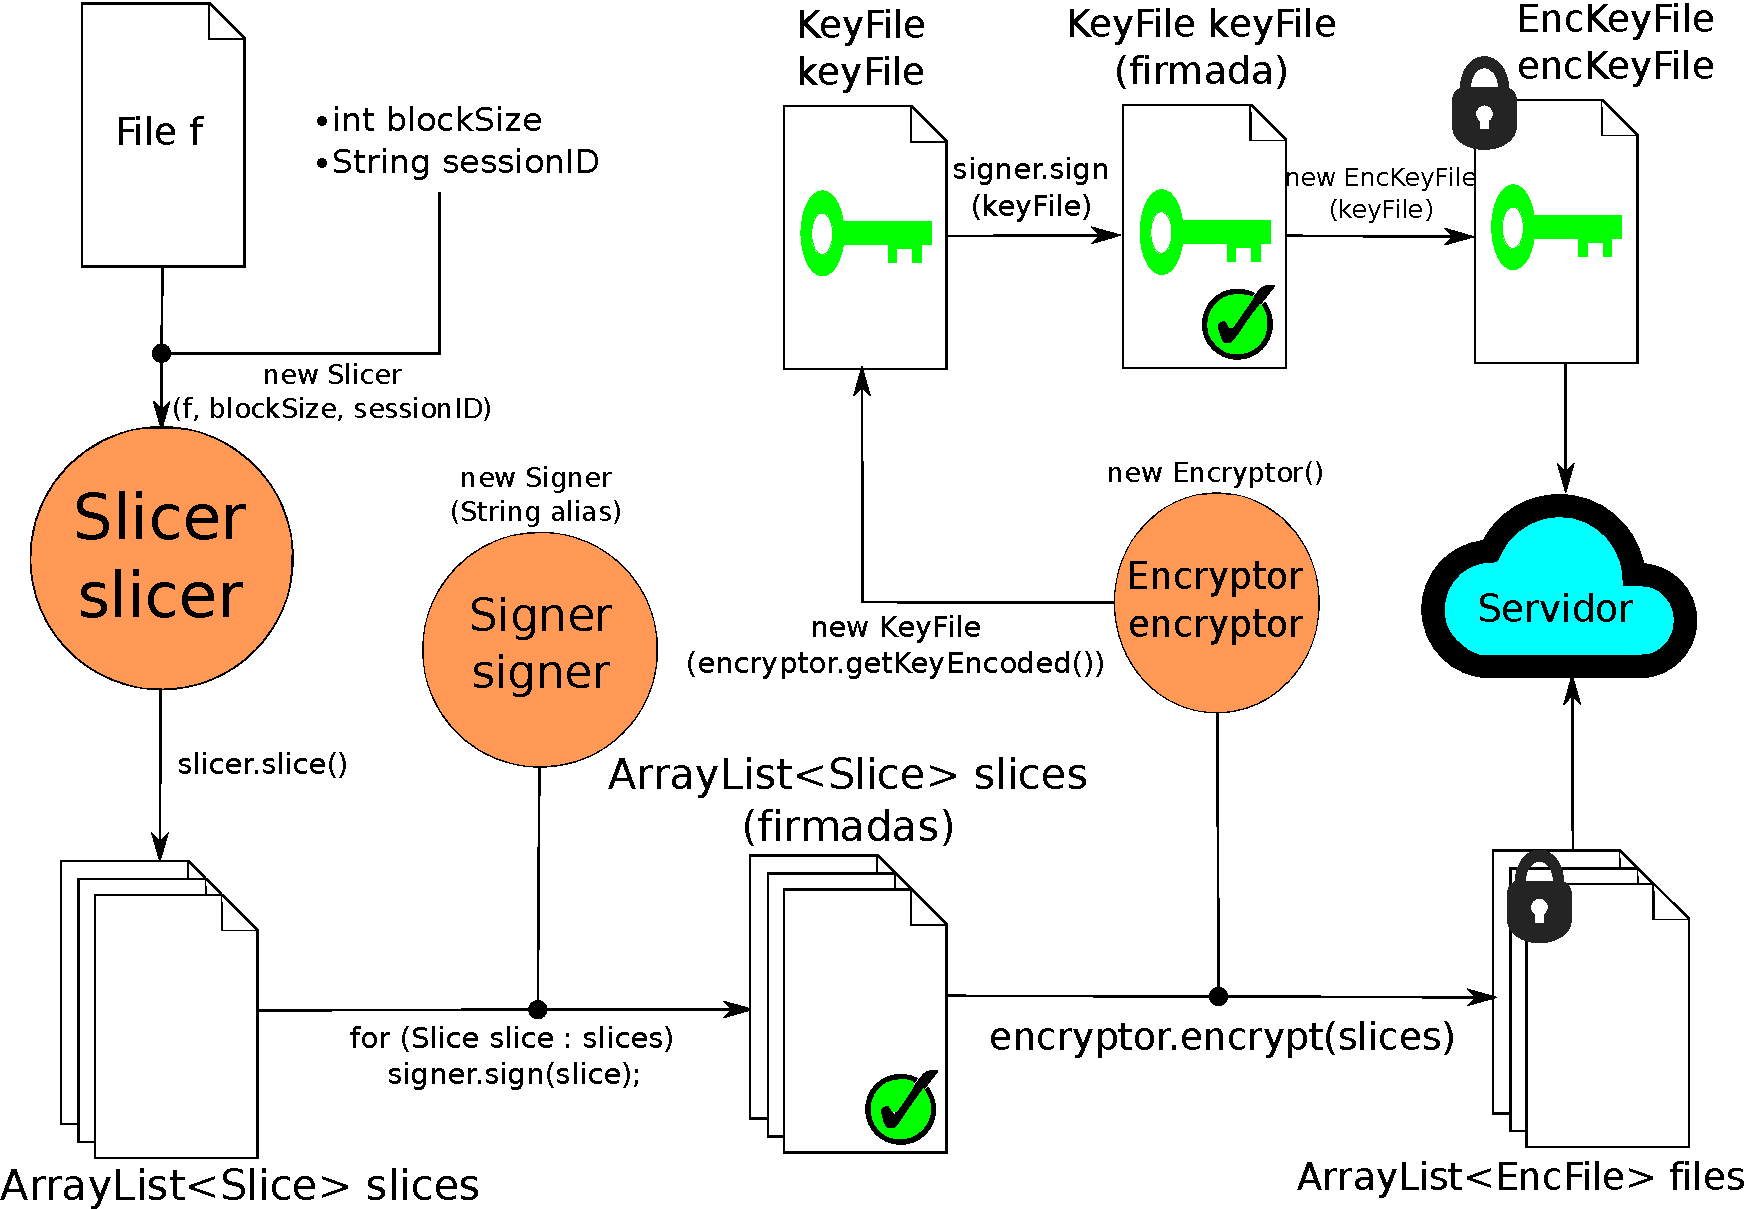
\includegraphics[scale=0.5]{Figures/abstractA}
  \decoRule
  \caption[Slice - Encrypt]{Esquema general de Slice - Encrypt, la primera parte en el proceso de comunicación de la aplicación}
  \label{fig:abstractA}
\end{figure}

\begin{figure}[!htb]
  \centering
  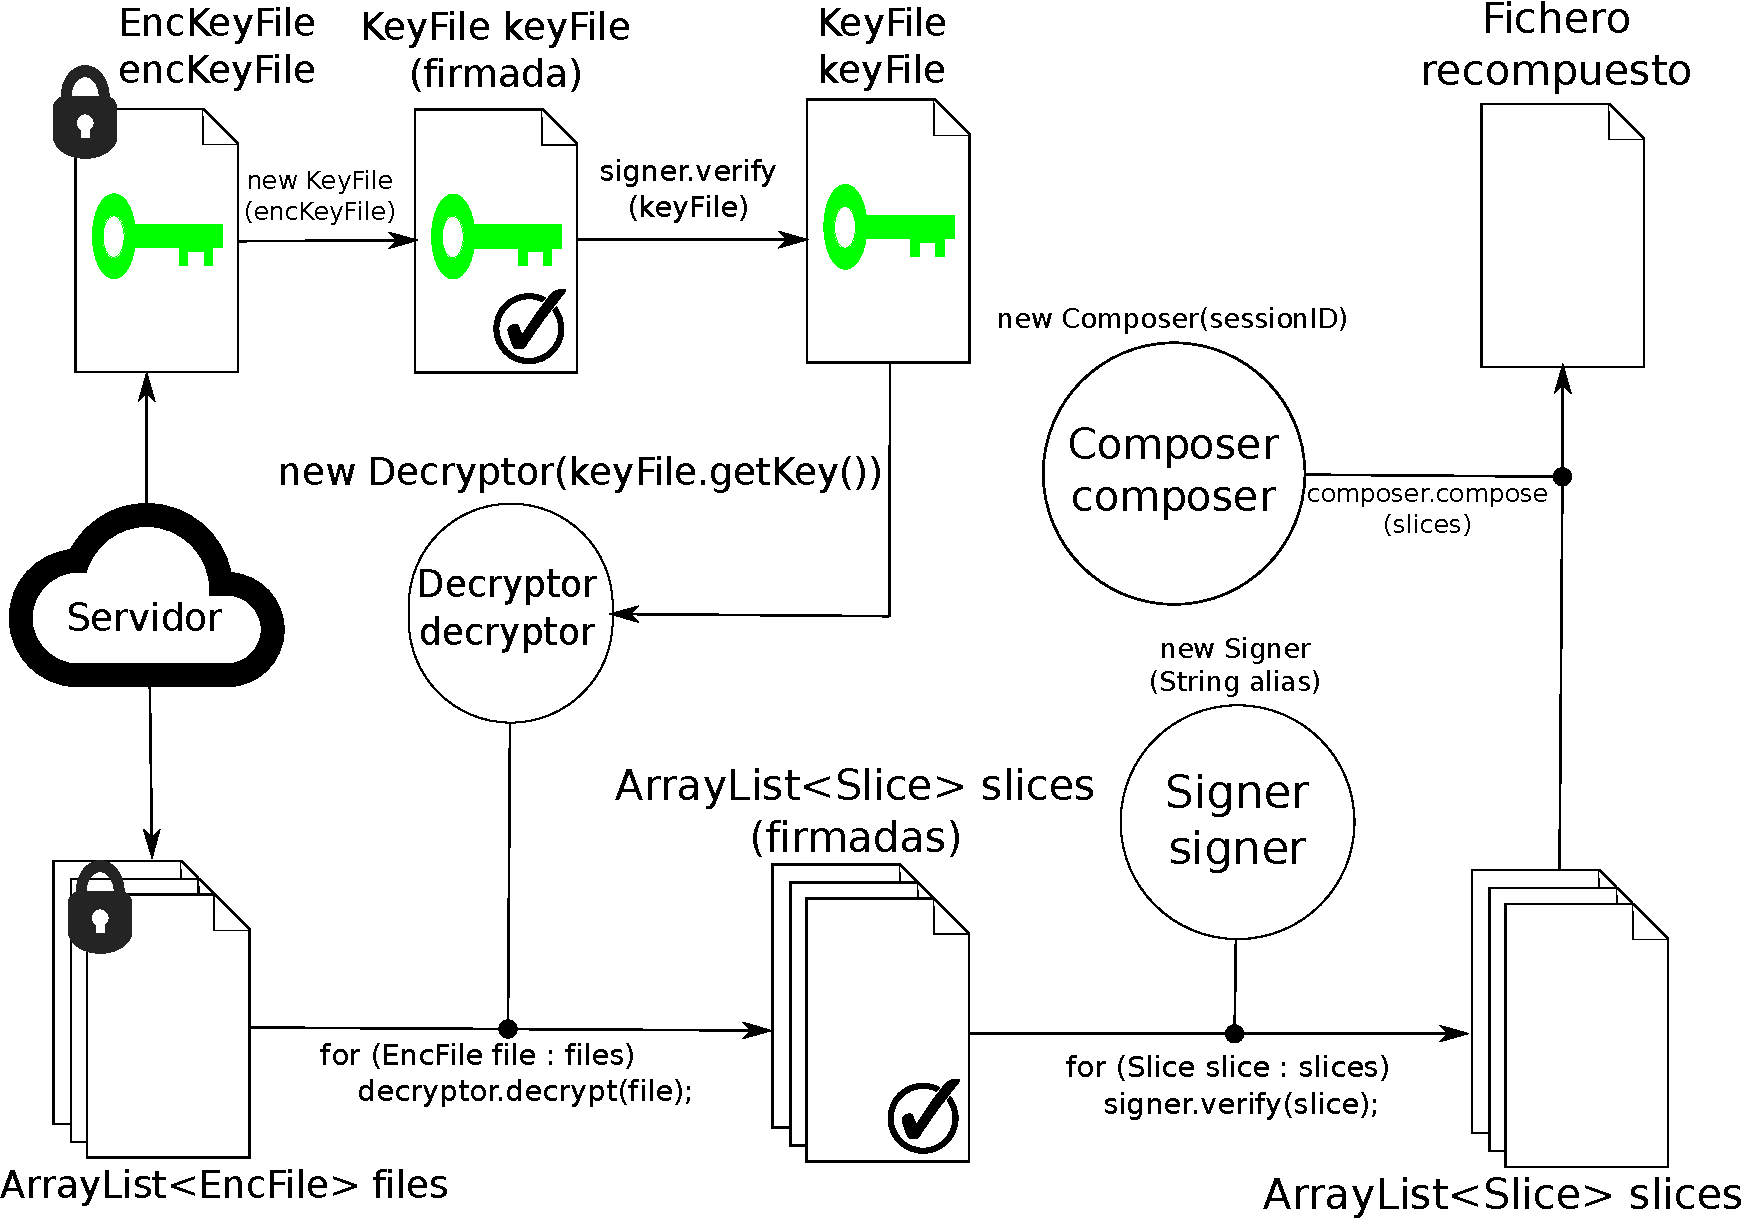
\includegraphics[scale=0.5]{Figures/abstractB}
  \decoRule
  \caption[Decrypt - Compose]{Esquema general de Decrypt - Compose, la parte final en el proceso de comunicación de la aplicación}
  \label{fig:abstractB}
\end{figure}
